\documentclass[aspectratio=169, 8 pt]{beamer}
\usepackage{pdfpages}
\usepackage{amsmath,amsthm,amssymb}
\usepackage{tikz}
\usepackage{pstricks}
\usepackage{ragged2e}
\usepackage{mathrsfs}
\usepackage{microtype}
\usepackage{bbm}
\usepackage{graphicx, wrapfig, subcaption, setspace, booktabs}
\usepackage{tabularx}
\usepackage{listings}
\usepackage{xcolor}
\usepackage{longtable}
%\usepackage{titlesec}
\usepackage{url, lipsum}
\usepackage{hyperref,bookmark}
\usepackage[T1]{fontenc}
\usepackage{amssymb}
\usepackage{tabularx}
\usepackage{listings}
\usepackage{xcolor}
\usepackage{longtable}
\usepackage{setspace}
\usepackage{float}
\usepackage{multirow}
\usepackage{tabularx}
\usepackage[at]{easylist}% easy lists with @ starting each item
\usepackage{algorithmic}
\usepackage{graphicx}
\usepackage{textcomp}
\usepackage{amsmath}
\usepackage[sc]{mathpazo}
\usepackage{datetime}
\usepackage{graphicx, wrapfig, subcaption, setspace, booktabs}
\usepackage[T1]{fontenc}
\usepackage{fourier}
\usepackage{url, lipsum}
\usepackage{hyperref,bookmark}
\usepackage[T1]{fontenc}
\usepackage{amssymb}
\usepackage{makecell, multirow, tabularx}
\usepackage{listings}
\usepackage[ruled,linesnumbered]{algorithm2e}

\usetheme{Pittsburgh}
\ifdefined\ishandout
	\usecolortheme{seagull}
\else
	\usecolortheme{scottybear}
\fi

\usefonttheme{serif}
\hypersetup{colorlinks,linkcolor=,urlcolor=links}

% Theorem Styles

\theoremstyle{theorem}
\newtheorem{thm}{Theorem}
\newtheorem{lm}{Lemma}
\newtheorem{ex}{Example}
\newtheorem{exs}{Examples}

\theoremstyle{definition}
\newtheorem{defn}{Definition}
\newtheorem{notation}{Notation}

\theoremstyle{remark}
\newtheorem*{remark}{Remark}

% Commands

\DeclareMathOperator{\diam}{diam}
\DeclareMathOperator{\id}{id}

\newcommand{\8}{\infty}
\newcommand{\A}{\mathscr{A}}
\newcommand{\C}{\mathbb{C}}
\newcommand{\N}{\mathbb{N}}
\newcommand{\Q}{\mathbb{Q}}
\newcommand{\R}{\mathbb{R}}
\newcommand{\Z}{\mathbb{Z}}
\newcommand{\iunit}{\mathbbm{i}}

\newcommand{\dif}{\mathrm{d}}
\newcommand{\diff}{\,\mathrm{d}}
\newcommand{\Dim}[1]{\dim_{\mathrm{#1}}}
\newcommand{\st}{\,|\,}
\newcommand{\ST}{\,\middle|\,}
\newcommand{\Poles}{\mathscr{P}}
\renewcommand\vec[1]{\boldsymbol{#1}}
\newcommand\Union{\mathop{\bigcup}}
\newcommand\Intersect{\mathop{\bigcap}}
\newcommand\union{\mathrel{\cup}}
\newcommand\intersect{\mathrel{\cap}}

\newgray{darkgrey}{.25}
\newgray{grey}{.5}
\newgray{lightgrey}{.75}
\newgray{vlightgrey}{.9}

\newcommand{\secslide}[2]{
	\section[#1]{#2}
		\begin{frame}
			\begin{center}
				\ifdefined\ishandout
					\textbf{\Huge\secname}
				\else
					\textcolor{structure}{\textbf{\Huge\secname}}
				\fi
			\end{center}
		\end{frame}
}

\renewcommand{\baselinestretch}{1.1}


\title[]{CO\textsubscript{2} and Cost Impacts of a Transportation-microgrid with Electric Vehicle Charging Infrastructure: a case study in Southern California}
\author[]{Luis Fernando Enriquez-Contreras}
\institute[]{University of California, Riverside}
\date{December 1, 2023}


\definecolor{codegreen}{rgb}{0,0.6,0}
\definecolor{codegray}{rgb}{0.5,0.5,0.5}
\definecolor{codepurple}{rgb}{0.58,0,0.82}
\definecolor{backcolour}{rgb}{0.95,0.95,0.92}

\lstdefinestyle{mystyle}{
	backgroundcolor=\color{backcolour},   
	commentstyle=\color{codegreen},
	keywordstyle=\color{magenta},
	numberstyle=\tiny\color{codegray},
	stringstyle=\color{codepurple},
	basicstyle=\ttfamily\footnotesize,
	breakatwhitespace=false,         
	breaklines=true,                 
	captionpos=b,                    
	keepspaces=true,                 
	numbers=left,                    
	numbersep=5pt,                  
	showspaces=false,                
	showstringspaces=false,
	showtabs=false,                  
	tabsize=2
}

\lstset{style=mystyle}

\begin{document}

\usebackgroundtemplate{
	\tikz[overlay,remember picture] \node[opacity=0.04, at=(current page.center), yshift=-1.1in, xshift=1.75in] {
   
\includegraphics[height=3in]{aux/ucr_seal_black.eps}};
}

% ----------------------------------------------------------------------
% TITLE SLIDE ----------------------------------------------------------
% ----------------------------------------------------------------------

\begin{frame}[plain] 
	\titlepage

	\ifdefined\ishandout
	  \newcommand{\LOGO}{aux/ucr_logo_grey.eps}
	\else
	  \newcommand{\LOGO}{aux/ucr_logo_cmyk.eps}
	\fi

	\begin{tikzpicture}[remember picture,overlay]
		\node[anchor=south west,yshift=2pt,xshift=4pt] at (current page.south west) {\includegraphics[height=1cm]{\LOGO}};
	\end{tikzpicture}
\end{frame}

% ----------------------------------------------------------------------
% OUTLINE --------------------------------------------------------------
% ----------------------------------------------------------------------

\begin{frame}{Outline}
	\vfill
	\tableofcontents
	\vfill
\end{frame}

% ----------------------------------------------------------------------
% FRAMES ---------------------------------------------------------------
% ----------------------------------------------------------------------

%	\secslide{Short Sec}{A section with a long title and a short tag}
%	\begin{frame}{\secname}
%		The macros \texttt{\textbackslash secslide} creates a new section (with an entry in the table of contents), and produces a nice title slide for the section.  This behaviour is defined in the \texttt{aux/macros.tex} file.  The \texttt{aux/} directory also contains some other useful files, such as a bibliography file and logos.
%	\end{frame}	
\section{Introduction}
	\begin{frame}
		\frametitle{Introduction}	
		\begin{itemize} \large
			\item Electrification of Transportation
				\begin{itemize} 
					\item Electric vehicle (EV) adoption is increasing rapidly, with 25.4\% of Q2 2023 vehicle sales being EVs in California
					\item California aims to ban the sale of internal combustion engine vehicles by 2035
					\item The state is expanding its EV charging infrastructure, with over 13,844 Level 2 and 1,924 Level 3 stations as of November 2023
					\item Technological advances allow new EVs to charge up to 80\% in 20-60 minutes, making EVs more appealing
					\item This rapid charging capability poses challenges for grid operators due to the high electricity demand it creates
				\end{itemize}
			\item Challenges
				\begin{itemize} 
					\item Two key challenges exist: 
					\begin{itemize} 
						\item Providing enough electricity capacity for the growing number of EVs
						\item Minimizing the CO\textsubscript{2} emissions associated with battery electric vehicles by ensuring a clean grid
					\end{itemize}
				\end{itemize}
			\item Solution
				\begin{itemize} 
					\item Microgrids offer a potential solution to both challenges
					\item Microgrids can integrate renewable energy sources and EV charging stations, reducing the burden on the main grid and minimizing CO\textsubscript{2} emissions
				\end{itemize}
			\item Research Focus
				\begin{itemize} 
					\item Further research is needed to understand the economic and environmental impacts of EV charging, especially fast charging, and how microgrids can be effectively utilized to manage EV demand and promote a sustainable transportation future
				\end{itemize}
		\end{itemize}
	\end{frame}
	\begin{frame}
		\frametitle{Contribution}
%		\begin{itemize}
%			\item analyze the impacts Zero-Emission Vehicles Infrastructure (Level 2 and
%			Level 3 charging) have on the behavior of microgrids and
%			the associated electric costs and CO2 emissions in southern
%			California
%			\item the simulation is run in system dynamics software as opposed to using data analytics software
%			\item a higher time resolution data is used to calculate CO2 emissions instead of average value
%		\end{itemize}
		\large
		\begin{itemize}
			\item This research holds significant implications for the advancement of intelligent transportation systems, as it aims to address the economic needs of EV charging infrastructure owners and determine the optimal configuration that benefits both EV owners and the environment by minimizing greenhouse gas emissions
			\item This paper delves into the impacts of transportation-microgrids equipped with Level 2 and Level 3 charging on the behavior of microgrids, associated electricity costs, and CO\textsubscript{2} emissions within the context of southern California
			\item The simulations are conducted using OpenModelica, a dynamic modeling and simulation environment
			\item This study distinguishes itself from previous research in many ways, including employing a higher time resolution for calculating CO\textsubscript{2} emissions that is measured every 15 minutes
		\end{itemize}
	\end{frame}
\section{Literature Review}

	\begin{frame}
		\frametitle{Transportation-Microgrids: Key Research Gaps}
		\Large
		\begin{itemize}
			\item Economic Analysis:
			\begin{itemize} \large
				\item Current focus on energy charges overlooks demand charges, crucial for fast charging stations
				\item A comprehensive approach considering both energy and demand charges is needed
			\end{itemize}
			\item Impact of EV Charging Demand:
			\begin{itemize} \large
				\item Existing research focuses on low-demand Level 2 charging
				\item Studies should incorporate a mix of Level 2 and Level 3 charging scenarios for a nuanced understanding
			\end{itemize}
			\item CO\textsubscript{2} Emissions Assessment:
			\begin{itemize} \large
				\item Simplified approaches using average CO\textsubscript{2} emissions neglect time-varying emissions
				\item More sophisticated calculations are needed to accurately represent the environmental impact
			\end{itemize}  
		\end{itemize}
	\end{frame}
	
%		\begin{frame}
%			\frametitle{Literature Review}
%			\begin{itemize}
%				\item [5] Optimal configuration and investment costs of EVCS with solar power are highly dependent on feed-in tariffs and solar irradiation
%				\item [5] CO2 emissions were calculated on a per year basis, not dealing with daily variations. Only energy charges were calculated, not demand costs.
%				\item [6] A control algorithm is proposed to minimize charging time, costs, or maximize renewable energy use.
%				\item [6] Charging loads were modeled using a uniform distribution during peak times, with only Level 2 charging at 3.3 kW
%				\item [7] An EV charging model was proposed that shifts charging events from high peak times to low peak times
%				\item [7] The proposed method did little to reduce peak load shaving, and solar production surplus may not be shifted to EVs due to low availability.\
%				\item [7] The dataset was limited to one week, with four EVs in a system with 10 buildings
%				\item [8] Multiple scenarios with different self-consumption rates were run, first comparing scenarios and then calculating emissions for each
%				\item [8] CO2 emissions were calculated from whole-life-cycle CO2 emissions without high time resolution
%				\item [9] The Non-dominated Sorting Genetic Algorithm-II (NSGA-II) was used to analyze four different responses with 0\%, 10\%, 20\%, and 30\% EV penetration and a Monte Carlo load profile
%				\item [9] CO2 calculations were not explained, and the specific impacts of Level 2 versus Level 3 charging were not shown
%				\item [10] Multiple microgrids were used to balance out EV charging within the system. Multi-objective energy management of multiple microgrids was used to orchestrate the operation. 
%			\end{itemize}
%		\end{frame}
		
\section{Methodology}

	\begin{frame}
		\frametitle{CO\textsubscript{2} Emissions}
		\begin{itemize} \Large
			\item California Independent System Operator (CAISO) CO\textsubscript{2} emission data $\frac{\frac{\textsubscript{m}TON\textsubscript{CO\textsubscript{2}}}{hour}}{Wh}$ with a 15 minute resolution is multiplied with the energy consumed during that period to calculate the amount of CO\textsubscript{2} produced in that time frame
			\item  This gives us an estimate of the amount of CO\textsubscript{2} emissions in $\textsubscript{m}TON\textsubscript{CO\textsubscript{2} } $ for every 15 minutes that is summed together to give us the total for the entire period
			\item When the grid does not pull power from the grid or is sending power, the CO\textsubscript{2} emissions are assumed to be
			zero since we are using our solar energy
		\end{itemize}

	\end{frame}

	\begin{frame}
		\frametitle{Microgrid Setup in OpenModelica}
		\begin{itemize} \large
			\item Modelica is a programming language designed for dynamic systems simulation
			\item OpenModelica is an open-source implementation of the Modelica programming language
			\item OMEdit is the GUI interface for OpenModelica, allowing the user to draw a system for simulation
			\item The microgrid scenarios are simulated in OpenModelica using the Modelica buildings library
			\item The Modelica buildings library was created by Lawrence Berkeley National Laboratory for building and district energy and control systems
			\item The library's capability for energy storage systems, bidirectional inverters, solar, and HVAC modeling makes it ideal for a microgrid simulation setup
			\item This allows us to create scenarios that do not currently exist in our microgrid, like running a month with solar with the same load or running the BESS control algorithm for different electric rates
			\item The simulation of our case study microgrid is the grid-connected to the building netload
			\item The model's net load is broken down into solar power, HVAC demands, regular building demands, electric vehicle chargers, and the BESS
		\end{itemize}
	\end{frame}
	
	\begin{frame}
		\frametitle{Microgrid Setup in OpenModelica}
		\begin{figure}
			\centering
			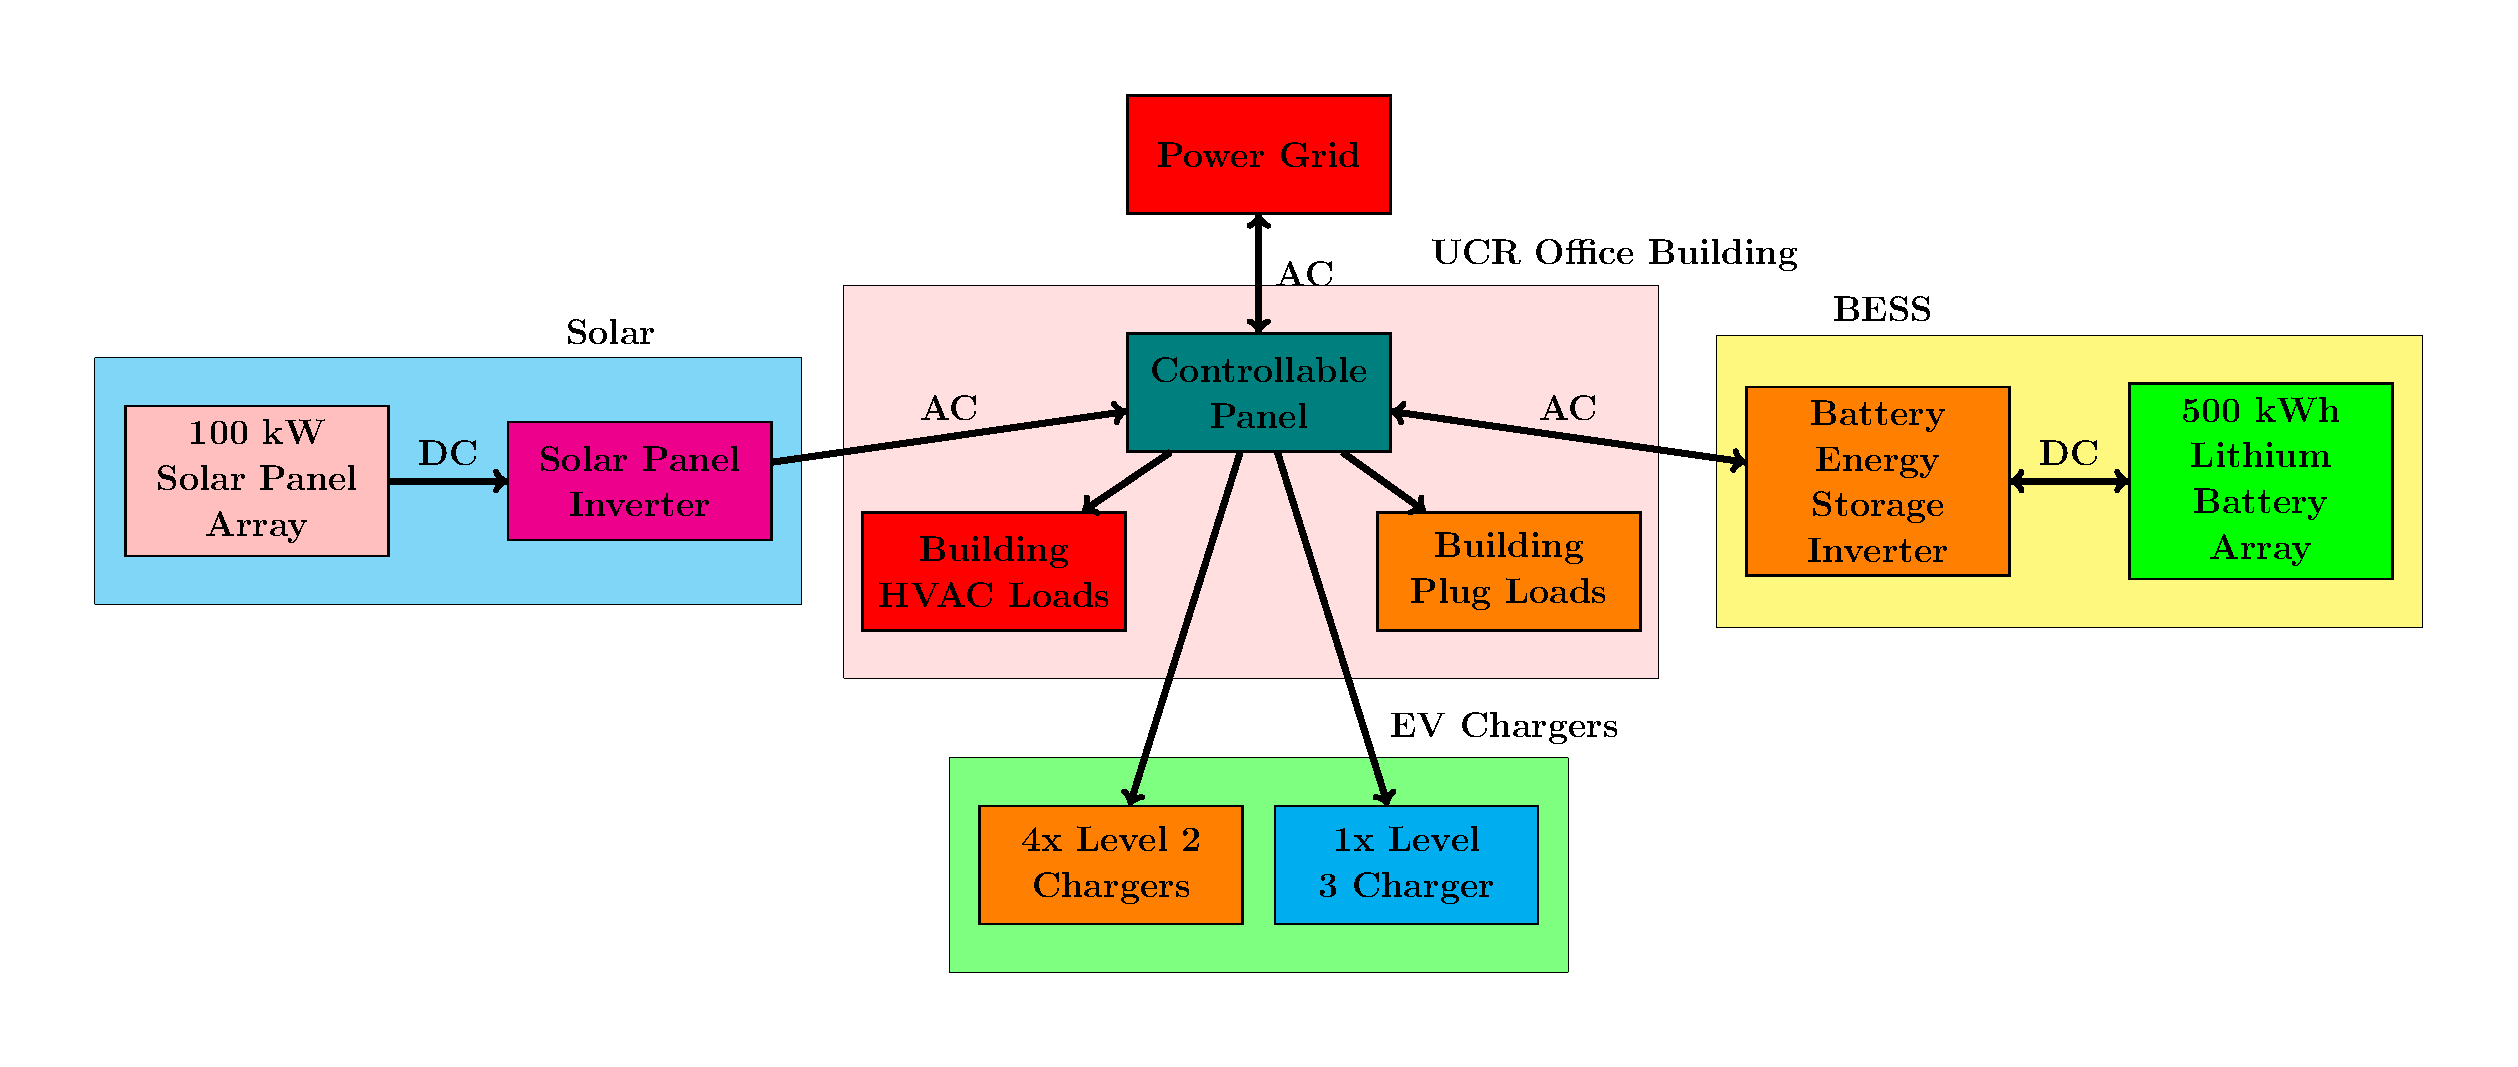
\includegraphics[width=0.9\linewidth]{Fig/power_system_setup_modelica_large}
			\caption{Microgrid Architecture of our Case Study Example BESS: Battery Energy Storage System}
			\label{fig:powersystemsetupfull}
		\end{figure}
	\end{frame}

	\begin{frame}
		\frametitle{Whole System Validation}
		\begin{itemize}
			\item To ensure that our model accurately portrays our real world system, a year of real world data was used to validate the $P_G $ output . $P_G$ is defined as the power the microgrid sends or consumes from the grid
			\item The actual data was compared to the simulated  with a correlation coefficient of  $\approx$ 0.965087 as shown in Figure \ref{fig:ucr15minutedatamar012022tomar012023}
		\end{itemize}
		\begin{figure}
			\centering
			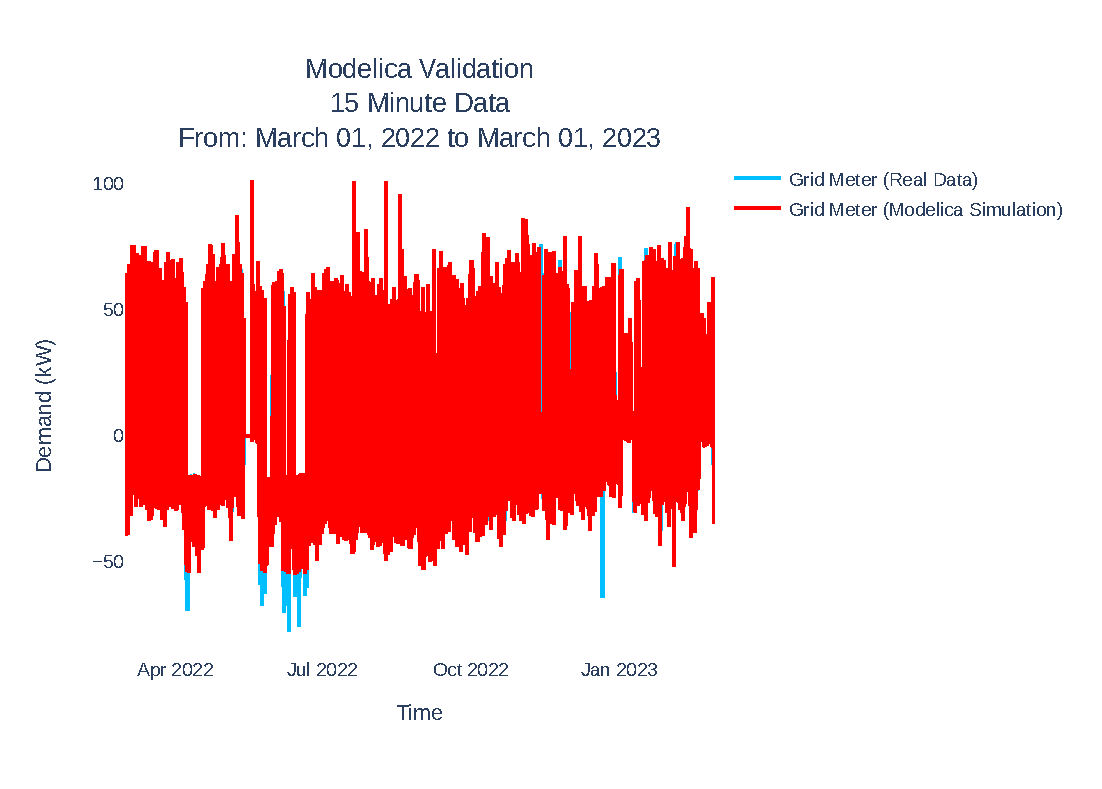
\includegraphics[width=0.55\linewidth]{Fig/ucr_15_Minute_Data_Mar_01_2022_to_Mar_01_2023}
			\caption{Whole Year Validation of the Microgrid Architecture in OpenModelica. The bright blue and red is the real data and simulated data respectively. The dark red is the overlap between real and simulated data.}
			\label{fig:ucr15minutedatamar012022tomar012023}
		\end{figure}		
	\end{frame}

	\begin{frame}
		\frametitle{EV Chargers Load}
%		\begin{itemize}
%			\item Our model also considers transportation loads in the form of EV chargers.
%			\item The EV chargers are represented as two models: Level 2 EV chargers, and Level 3 EV chargers.
%			\item While other loads follow a typical daily and yearly pattern, EV loads are different since they switch on and off.
%			\item Our case study microgrid has four Level 2 chargers, so it can have four ``steps'' of 7.2 kW each, while there is only one ``step'' of 50 kW with the Level 3 chargers.
%			\item To generate EV loads, we use a Poisson random generator to generate the number of charge sessions in a day, the arrival times, and charging durations based on real world data.
%			[Image of Poisson random generator]
%		\end{itemize}
		
		\begin{itemize} \large
			\item EV chargers are represented as two models: Level 2 EV chargers, and Level 3 EV chargers.
			\item The case study microgrid has four Level 2 chargers, so it can have four “steps” of 7.2 kW each, while there is only one “step” of 50 kW with the Level 3 chargers
			\item Historical data from the Level-2 charger was utilized to determine the parameters for the Poisson random generator, consistent with the typical daily charge probability density function (PDF).
			\item Analysis of the historical data revealed three distinct peak charging periods occurring at 7:00, 9:00, 13:00, with average number of vehicle arrivals during each peak of 6, 2, and 1 respectively
			\item A mean charging time of 90 minutes was assumed
			\item The EV random arrivals function generates random arrival times and durations
			\item The function employs the NumPy library in Python to create a Poisson random distribution with means centered around the peak times.
			\item To ensure consistency across different scenarios and prevent any outlier event from the EV charging load disproportionately influencing higher demand events, a random data seed value of 10 was employed to ensure every charging event is the same
			\item The random arrivals for Level 3 charging are modeled with three peak times at 7:00, 9:00, 13:00, an average vehicle arrival count of 2, 1, and 1, and a mean charging time of 30 minutes
		\end{itemize}
	\end{frame}

		\begin{frame}
			\frametitle{EV Chargers Load}
			\begin{figure}
				\centering
				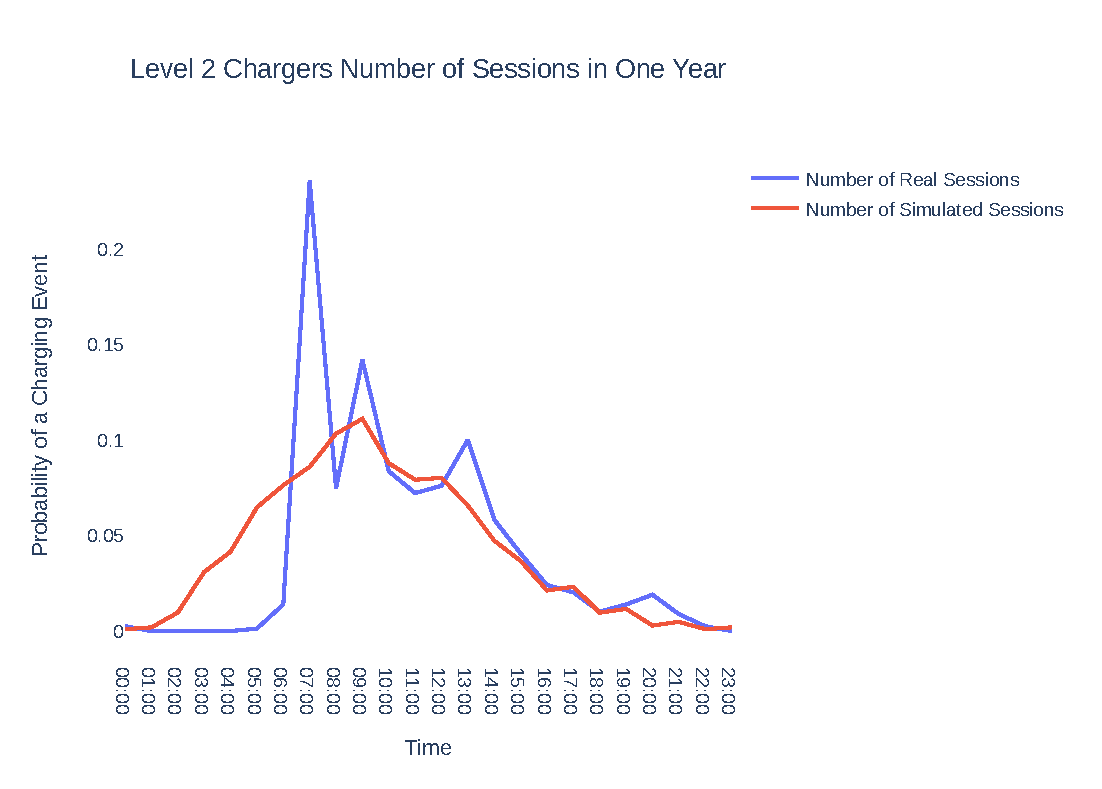
\includegraphics[width=0.7\linewidth]{Fig/l2_avg_day_rand_poisson_1_hour_pdf}
				\caption{Validation of the Level 2 EV Charger Stochastic Process that Compares the Probability Density Function of Actual Charging Data to the Poisson Process}
				\label{fig:l2avgdayrandpoisson1hourpdf}
			\end{figure}
		\end{frame}
	
		\begin{frame}
			\frametitle{EV Chargers Load}
			\begin{figure}
				\centering
				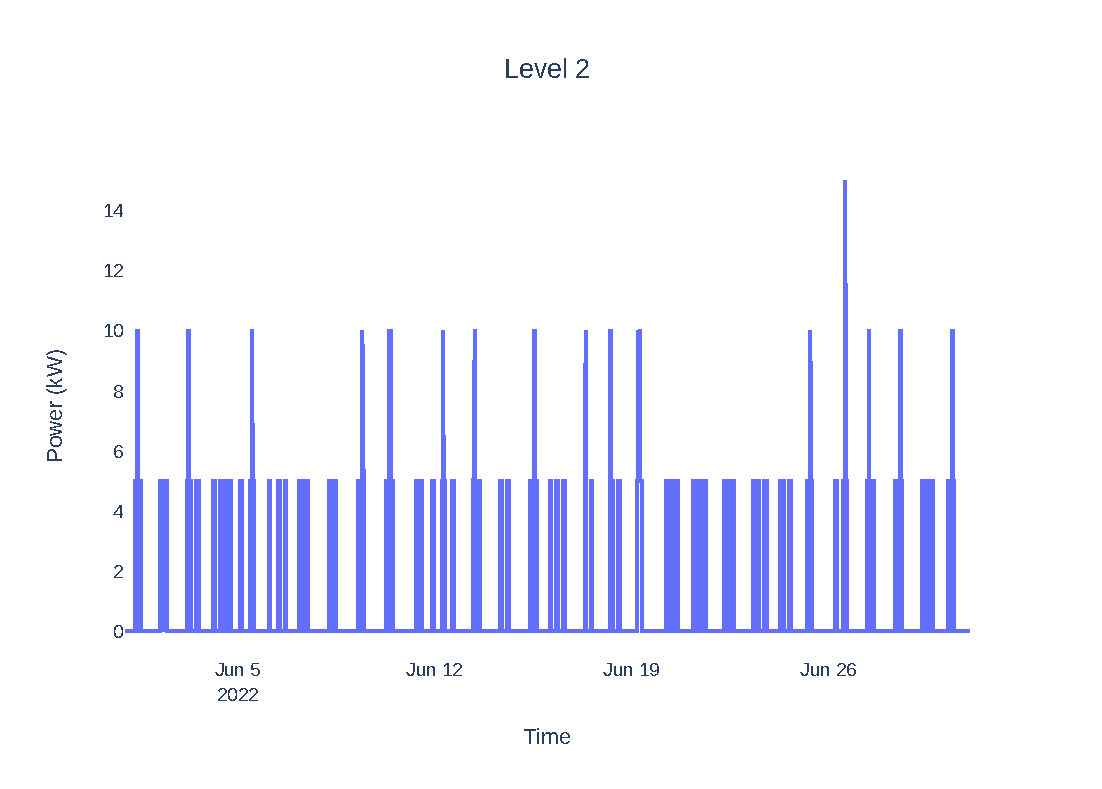
\includegraphics[width=0.7\linewidth]{Fig/l2_g_pad_poisson_June}
				\caption{Example Level 2 Chargers Simulated Power Draw in OpenModelica}
				\label{fig:l2gpadpoissonjune}
			\end{figure}
		\end{frame}
	
%		\begin{frame}
%			\frametitle{BESS and Peak Shaving}
%		
%			Algorithm 1 shows the peak shaving algorithm sufficient for flat rate demand response.
%			
%			\begin{figure}
%				\centering
%				\includegraphics[width=0.65\linewidth]{Fig/peak}
%				\caption{}
%				\label{fig:peak}
%			\end{figure}
%		\end{frame}
\section{Results}	
		\begin{frame}
			\frametitle{Results}
			\begin{itemize}
				\item The charging setup is modified in OpenModelica for different layouts and scenarios
				\item The scenarios are described in Table \ref{tab:scenarios}
			\end{itemize}
			
			\begin{table}
				\caption{Simulated Scenarios of the UCR Microgrid using Different Layouts and Electric Pricing Structures}
				\large
				\begin{tabularx}{\linewidth}{l | l}
\toprule
 Scenario &  \\
\midrule
		1  & Standard Building with no EV Chargers\\
        2 & Standard Building with Level 2 and Level 3 Charging\\
        3 & Microgrid Building with 100 kW Solar, 500 kWh BESS, No EV Charging \\
        4 & Microgrid Building with 100 kW Solar, 100 kWh BESS, Level 2, and Level 3 Charging\\
        5 & Microgrid Building with 100 kW Solar, 250 kWh BESS, Level 2, and Level 3 Charging\\
        6 & Microgrid Building with 100 kW Solar, 500 kWh BESS, Level 2, and Level 3 Charging\\
        7 & Microgrid Building with 100 kW Solar, 1 MWh BESS, Level 2, and Level 3 Charging\\
        8 & Microgrid Building with 100 kW Solar, 1 MWh BESS, Level 2, and Level 3 Charging\\
\bottomrule
\end{tabularx}

				\label{tab:scenarios}
			\end{table}
		\end{frame}
	
		\begin{frame}
			\frametitle{Results}
			\begin{itemize}
				\item The charging setup is modified in OpenModelica for different layouts and scenarios
%				\item The scenarios are described in Table \ref{tab:scenarios}, Scenario 1 is the baseline case, Scenario 2 is the case where a building installs four Level 2 and one Level 3 charger, Scenarios 3 and 4 represents a transportation microgrid that has solar power and a 500kWh and 1000 kWh BESS for peak shaving respectively
				\item Each scenario is run independently of each other, and the power outputs of the different components in the simulation are shown in Figures \ref{fig:scenariospoweroutputboxplot}, \ref{fig:0scnoutputrun2mar012022tomar312022}, \ref{fig:4scnoutputrun2jul012022tojul312022}
				\item Scenarios 1 and 2 are both constantly negative meaning they are constantly pulling power from the grid
				\item Scenarios 3-8on the other hand is mostly positive or limited to -15, meaning it's either exporting power to the grid or it's consuming only 15 kilowatts
				\item The reason for the 15 kilowatt floor is because with the utility companies electric rate a minimum of 15 kilowatts is charged for the demand, meaning that a zero demand microgrid will not make a financial difference for the user
				\item The box plots show that all three figures mean and 75th percentile are almost identical at 15 kW. This implies that peak shaving is functioning correctly most of the time.
				\item However, the outliers show when the BESS fails to keep the power pulled from the grid at 15 kW
				\item Just one outlier will change the demand charge for the entire billing month
				\item Battery capacity affects the frequency of depletion and the ability to manage low-solar events
				\item Transportation-microgrids have lower CO\textsubscript{3} emissions than a conventional building, even with EV charging
				\item Adding EV charging increases CO\textsubscript{2} emissions by 17-45\% compared to a microgrid without EV chargers, but these emissions are offset by charging an average of 12 EVs per day
			\end{itemize}
			
		\end{frame}
		
	
		\begin{frame}
			\frametitle{Results}
			\begin{figure}
				\centering
				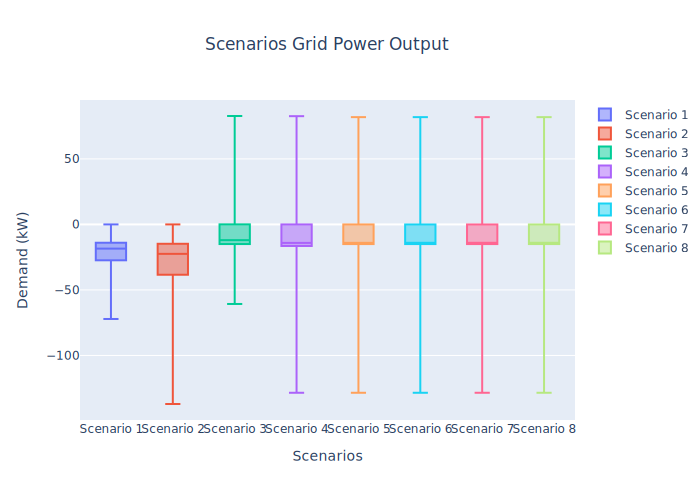
\includegraphics[width=0.7\linewidth]{Fig/scenarios_power_output_boxplot}
				\caption{Power measured from the meter}
				\label{fig:scenariospoweroutputboxplot}
			\end{figure}
		\end{frame}
		\begin{frame}
			\frametitle{Results}
			\begin{figure}
				\centering
				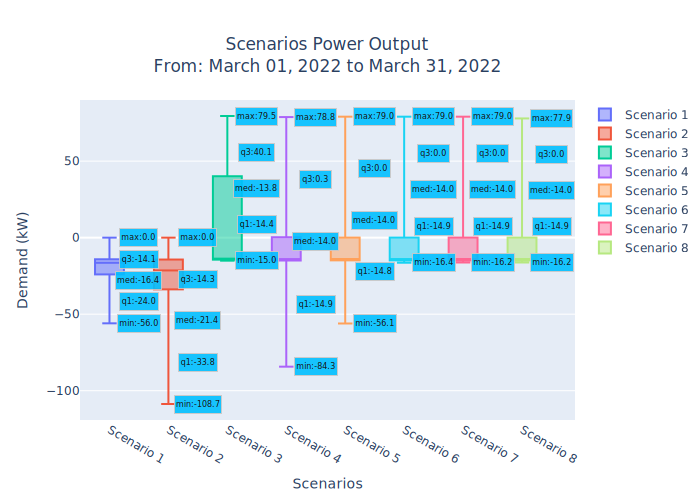
\includegraphics[width=0.7\linewidth]{Fig/0_Scn_Output_Run_3_Mar_01_2022_to_Mar_31_2022}
				\caption{Power measured from the meter for the month of March}
				\label{fig:0scnoutputrun2mar012022tomar312022}
			\end{figure}
		\end{frame}
		\begin{frame}
			\frametitle{Results}
			\begin{figure}
				\centering
				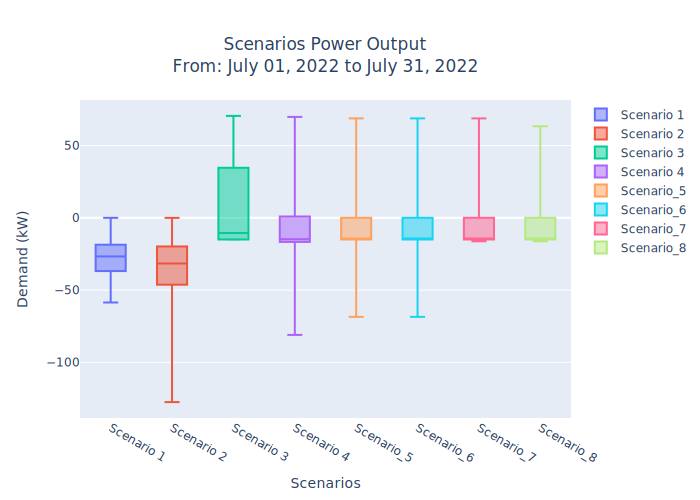
\includegraphics[width=0.7\linewidth]{Fig/4_Scn_Output_Run_3_Jul_01_2022_to_Jul_31_2022}
				\caption{Power measured from the meter for the month of July}
				\label{fig:4scnoutputrun2jul012022tojul312022}
			\end{figure}
		\end{frame}
%		\begin{frame}
%			\frametitle{Results}
%			\begin{figure}
%				\centering
%				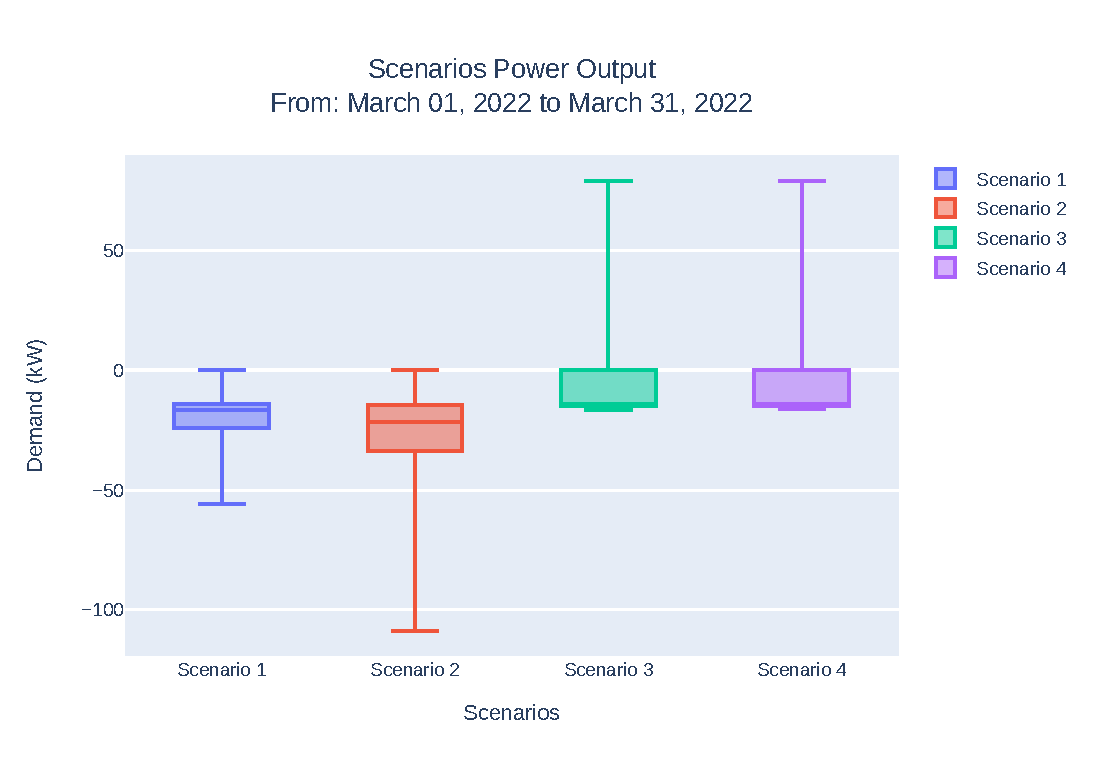
\includegraphics[width=0.7\linewidth]{Fig/0_Scn_Output_Run_2_Mar_01_2022_to_Mar_31_2022}
%				\caption{}
%				\label{fig:0scnoutputrun2mar012022tomar312022}
%			\end{figure}
%		\end{frame}
%	
%		\begin{frame}
%			\frametitle{Results}
%			\begin{figure}
%				\centering
%				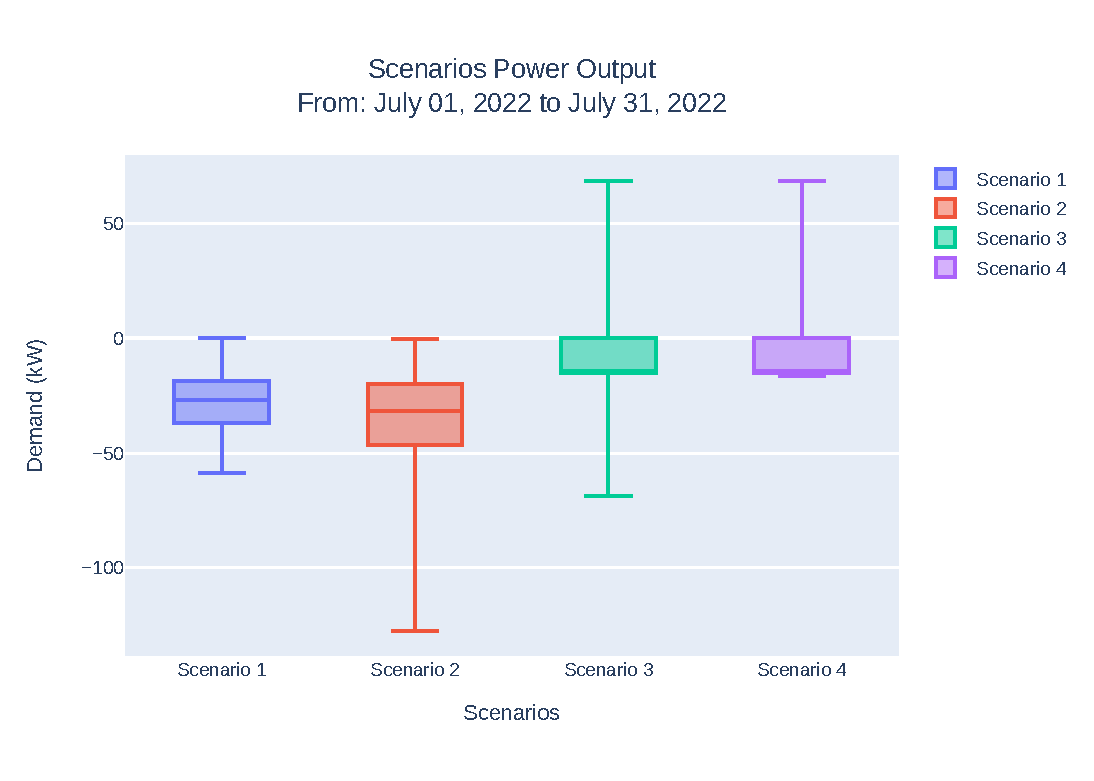
\includegraphics[width=0.7\linewidth]{Fig/4_Scn_Output_Run_2_Jul_01_2022_to_Jul_31_2022}
%				\caption{}
%				\label{fig:4scnoutputrun2jul012022tojul312022}
%			\end{figure}
%		\end{frame}
	
%		\begin{frame}
%			\frametitle{Results}
%			\begin{figure}
%				\centering
%				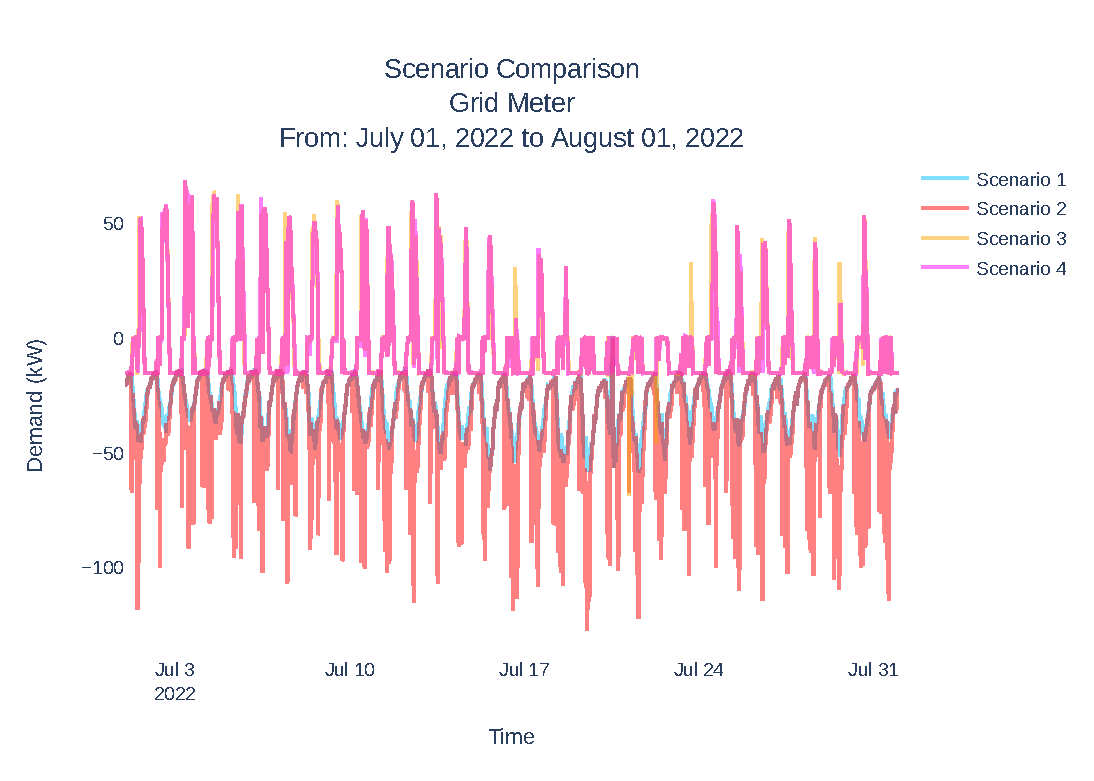
\includegraphics[width=0.7\linewidth]{Fig/net_load_scenario_comparison_summer_run_2}
%				\caption{Summer Net Load Scenario Comparison}
%				\label{fig:netloadscenariocomparisonsummer}
%			\end{figure}
%		\end{frame}
	
		\begin{frame}
			\frametitle{Results}
			\begin{figure}
				\centering
				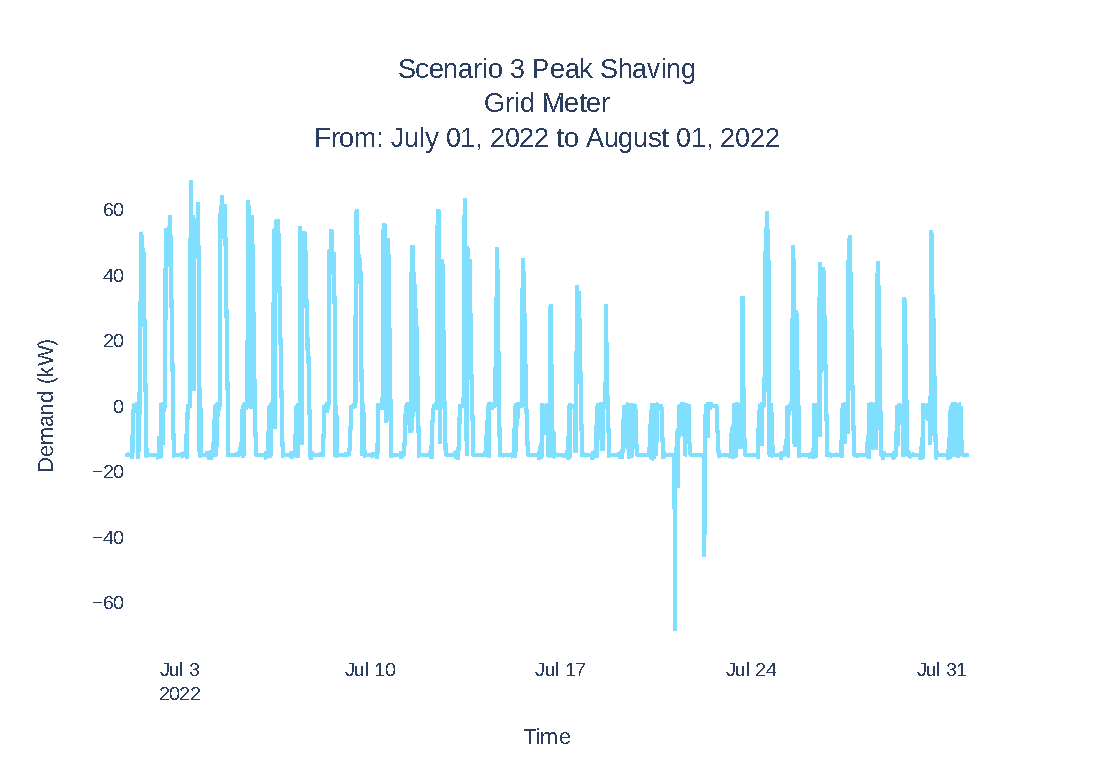
\includegraphics[width=0.7\linewidth]{Fig/scenario_3_peak_shaving}
				\caption{Peak Shaving Failure after Battery Depletion (500 kWh)}
				\label{fig:scenario3peakshaving}
			\end{figure}
		\end{frame}
	
		\begin{frame}
			\frametitle{Results}
			\begin{figure}
				\centering
				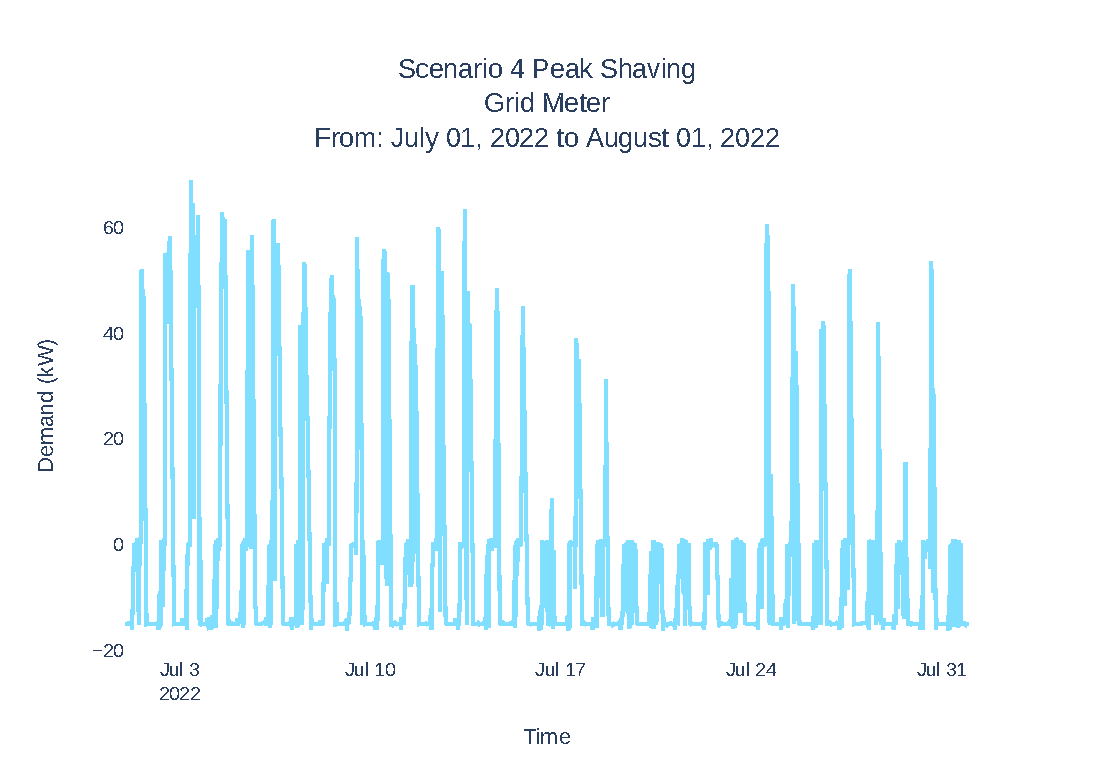
\includegraphics[width=0.7\linewidth]{Fig/scenario_4_peak_shaving}
				\caption{Peak Shaving Success with 1 MWh battery}
				\label{fig:scenario4peakshaving}
			\end{figure}
			
		\end{frame}
	
		\begin{frame}
			\frametitle{Results}
			\begin{figure}
				\centering
				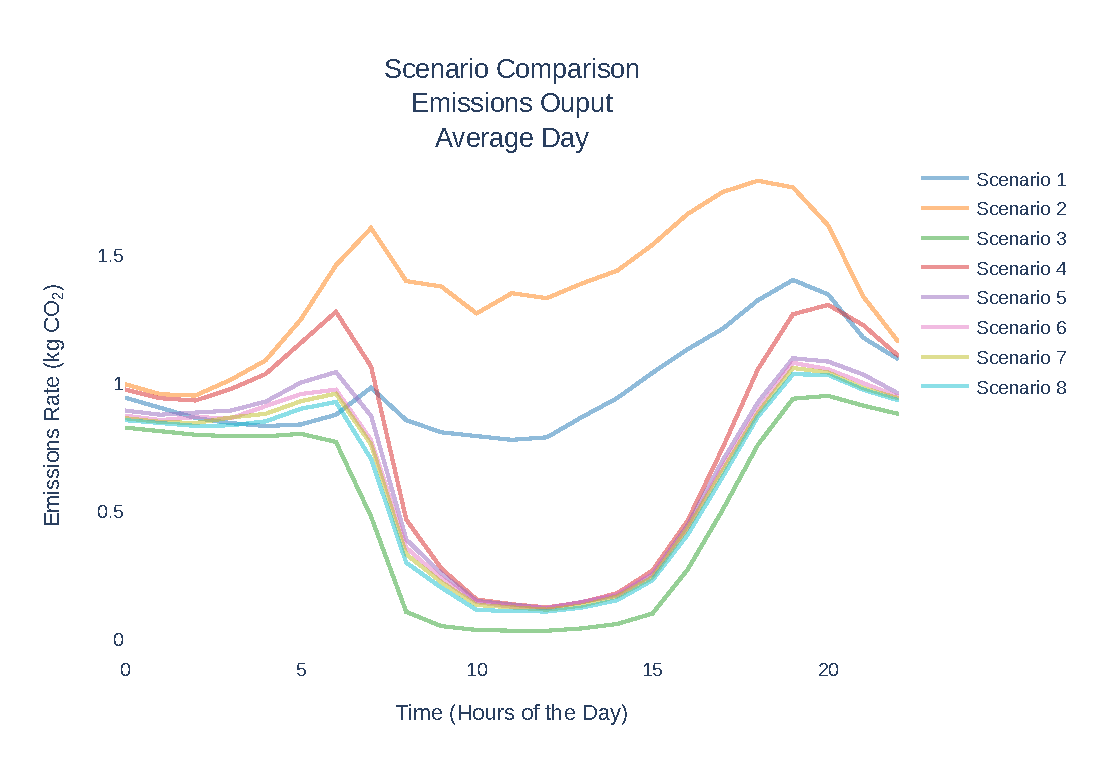
\includegraphics[width=0.7\linewidth]{Fig/emissions_scenario_comparison_run_3}
				\caption{Microgrid  CO\textsubscript{2} Emissions Outputs Averages During Times of Day}
				\label{fig:emissionsscenariocomparison}
			\end{figure}
		\end{frame}
	
		\begin{frame}
			\frametitle{Results}
			\begin{table}
				\caption{Microgrid Utility Prices and CO\textsubscript{2} Emissions Output under Different Pricing Scenarios and Pricing Structures}
				\centering
				\input{Table/kw_kwh_CO2_run_4.tex}
				\label{tab:emissions}
			\end{table}
		\end{frame}
	
		\begin{frame}
			\frametitle{Results}
			\begin{figure}
				\centering
				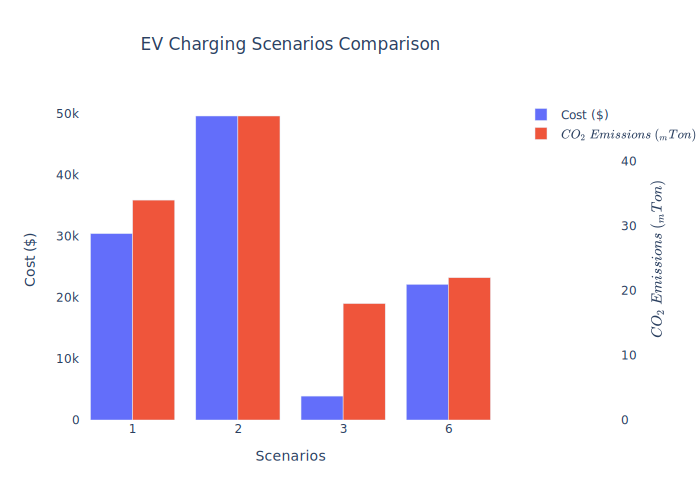
\includegraphics[width=0.7\linewidth]{Fig/mg_scene_comparison}
				\caption{EV Charging Scenarios Comparison}
				\label{fig:mgscenecomparison}
			\end{figure}
		\end{frame}
	
		\begin{frame}
			\frametitle{Results}
			\begin{figure}
				\centering
				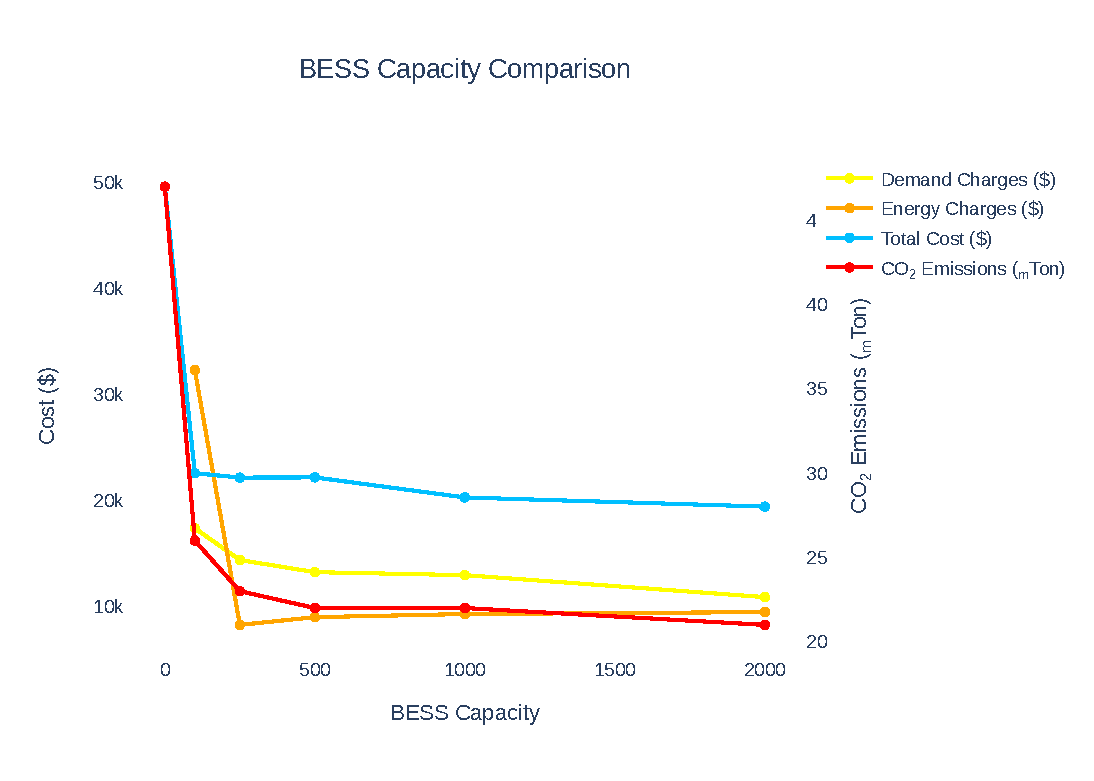
\includegraphics[width=0.7\linewidth]{Fig/bess_capacity_comparison}
				\caption{Cost and CO\textsubscript{2} Emissions for Different Battery Capacities}
				\label{fig:besscapacitycomparison}
			\end{figure}
		\end{frame}
	

		\begin{frame}
			\frametitle{Conclusion}
			\begin{itemize} \Large
				\item Transportation-microgrids offer significant economic and environmental benefits
					\begin{itemize} \large
						\item Estimated annual savings of \$8,000-\$10,000 compared to conventional systems
						\item Annual savings of \$27,000-\$29,000 compared to buildings with EV chargers but no microgrid
						\item 24\% - 38\% reduction in CO\textsubscript{2} emissions compared to conventional buildings
						\item 45\% - 55\% reduction in CO\textsubscript{2} emissions compared to buildings with EV chargers and no microgrid
					\end{itemize}
				\item Increased battery capacity does not guarantee improved performance
					\begin{itemize} \large
						\item Increased capacity improves performance but not proportionally to the cost
						\item Large capacity needed for challenging situations may not be cost-effective 
					\end{itemize}
				\item 15 kW demand price floor discourages zero net load
					\begin{itemize} \large
						\item Discourages zero net load in peak shaving setups, increasing CO\textsubscript{2} emissions
					\end{itemize}
				\item Future Work
					\begin{itemize} \large
						\item Optimizing electric costs and CO\textsubscript{2} emissions through throttling charging, maximizing solar energy use, and minimizing grid draw during peak CO\textsubscript{2} emissions times
						\item Assessing the impact of California's new net energy metering policy
					\end{itemize}
			\end{itemize}
%			\begin{itemize}
%				\item Transportation microgrids are an innovative solution for reducing the electric costs and emission levels of an EV charging setup
%				\item A comparative analysis of different scenarios shows that a transportation microgrid can offer significant savings and CO\textsubscript{2} over a conventional system
%				\item For a 100 kW 500 kWh transportation microgrid system, the annual savings are estimated to be \$8,000 a year or \$80,000 over a 10-year battery lifetime, even with additional demand from EV chargers
%				\item Compared to a building that installs EV chargers without a microgrid, the annual savings are even more substantial, reaching \$27,000 a year or \$270,000 over a 10-year battery lifetime
%				\item The transportation microgrid can reduce the CO\textsubscript{2} emissions by more than 50\% compared to the conventional building and by about 67\% compared to the scenario where the microgrid does not supply the building with clean energy
%				\item Increasing the battery capacity does not necessarily improve the performance of the microgrid. Doubling the battery capacity can eliminate some peaks from a couple of cloudy days, but the additional savings of \$2,000 per year do not justify the cost of the extra capacity
%				\item A 15 kW demand price floor has a negative impact on CO\textsubscript{2} emissions, as it discourages the user from maintaining the net load at zero in a peak shaving setup
%				\item Future research will explore different, more advanced control strategies to optimize the electric costs and CO\textsubscript{2} emissions of the transportation microgrid
%				\item The effects of the new net energy metering policy in California on the value of the BESS system will also be assessed
%				\end{itemize}			
		\end{frame}
		
	
	
\end{document}
